\chapter{Antecedentes} \label{cap:antecedentes}

\section{Motores de combustión interna}

% Estas son las ideas que quiero escribir aca

Introducción e importancia de seguir mejorando los diseños de motores, van a
estar funcionando un largo tiempo y hay que cuidar las emisiones etc.

Los motores de combustión interna son máquinas cuyo propósito es convertir la
energía química del combustible en energía mecánica.

Hay que seguir desarrollándolos y mejorándolos porque van a seguir estando
mucho tiempo.

Es importante mejorar la eficiencia de los sistemas de intercambio de gases
porque limitan la producción de potencia del motor

\subsection{Simulación del ciclo}
%

Modelo termodinámico, combustión a volumen constante y a presión constante.
%
Modelo de gases.



\subsection{Sistema de intercambio de gases}
%
El sistema de intercambio de gases cumple la función de extraer los gases
quemados de la cámara de combustión de manera eficiente al final de cada
carrera de expansión, además se encarga de admitir una carga de mezcla frezca a
la cámara de combustión para el próximo ciclo.
%
En un motor de cuatro tiempos, este sistema suele estar compuesto por un filtro
de aire, un tubo que conecta el filtro con el cuerpo de mariposa, el cuerpo de
mariposa, un plenum de admisión y un puerto de admisión, como se ve en la
figura \ref{fig:sist_intercambio}. 
%
La cantidad de aire inducatdo limita la cantidad de combustible que se puede
quemar, por este motivo es imporatnte tener un sistema de admisión eficiente.
%
De misma manera, la cantidad de gases quemados que se pueden extraer luego de
cada ciclo limita la cantidad de masa fresca que puede ingresar a la cámara de
combustión.
%
Otros objetivos de del sistema de intercambio de gases son el de preparar la
mezcla\footnote{En el caso de motores SI que admiten mezclas de aire y
combustible} y brindar un flujo que favorezca el proceso de combustión.

\begin{figure}[h!] \centering
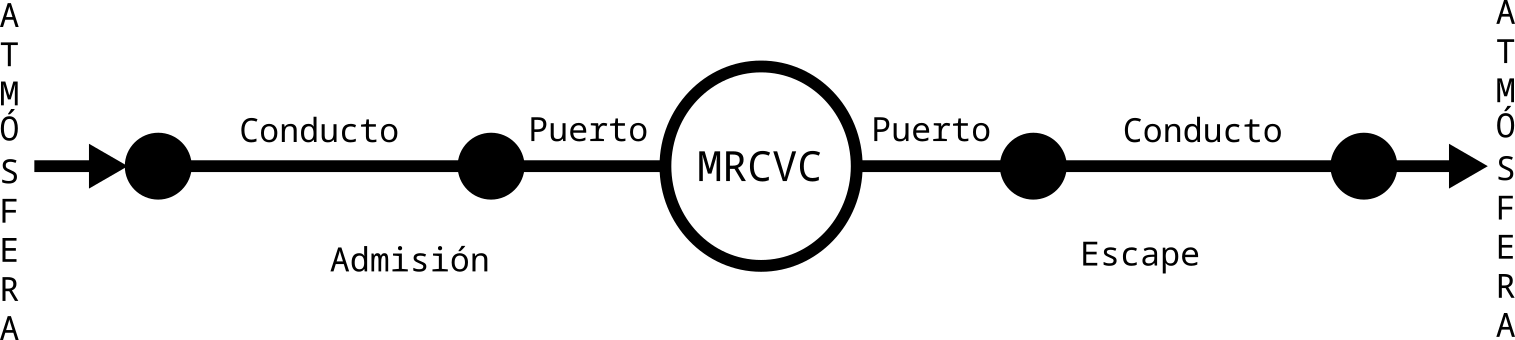
\includegraphics[width=0.5\textwidth]{sistema_intercambio_gases.png}
\caption{Sistema de intercambio de gases esquematizado(buscar una libre o hacer
un esquema propio)} \label{fig:sist_intercambio} \end{figure}

Para la simulación del MRCVC se usa una sistema simplificado, que consta de un
tubo de diámetro $D$ y longitud $L$ tanto para la admisión como para el escape,
como se ilustra en la figura \ref{fig:sist_int_mrcvc}.
%
La apertura y cierre de los puertos es controlada por la posición de los
puertos en el estator.

\subsection{Renidimiento Volumétrico} \label{sec:rend_vol}
%
% Por qué es importante este parámetro.

Los conductos de admision restringen el flujo de aire hacia el motor, para
medira la eficiencia con la que se está admitiendo aire al motor se define el
rendimiento volumétrico $\eta_v$.
%
Se define como la relación entre el caudal volumétrico de aire que ingresa al
sistema de admisión y la velocidad a la que cambia el volumen dentro de un
cilindro.


$$ \eta_v = \frac{2 \dot{m}_a}{\rho_{a,i} V_d N} $$

Donde: $\rho_{a,i}$ es la densidad del aire a la entrada del sistema de
admisión (para motres naturallmente aspirados). También se puede definir
$\eta_v$ como:

$$ \eta_v = \frac{m_a}{\rho_{a,i} V_d} $$

Dónde $m_a$ es la masa inductada al cilindro por ciclo.

Hay varios factores que afectan al rendimiento volumétrico, entre los más
importantes están:
%
\begin{enumerate} \item Efectos cuasiestáticos \item Pérdidas de carga por
    fricción viscosa \item Périddas de carga en los puertos de admision y
    escape \item Transferencia de calor en sistema de admisión \item Reglaje de
    los válvulas/puertos \item Bloqueos de flujo en puertos de admisión y
    escape \item Transferencia de calor en el cilindro \item Sintonía del
    puerto de admisión y escape \item Métodos de sobrecarga \end{enumerate}

Para este trabajo es de interés particular la pérdida de carga en los puertos,
el reglaje y la sintonía de en la admisión y escape.
%
En \cite{lopez13} se demostró que se tiene una mejor \emph{performance} del
motor si se ubican los puertos en el cuerpo central del estator, realizando un
optimzación previa de la geometría mediante un barrido paramétrico de las
variables geométricas que determinan la forma, posición y reglaje de los
puertos.
%
% La ubicación angular de los puertos determina la duración de los procesos de
% admisión y escape, además de modificar la forma y el coeficiente de descarga.

Todos estos parámetros se ajustan o tienen en cuenta con un objetivo de motor
en específico, por lo que fue necesario establecer una curva de renidmiento
volumétrico a la que aspirar para que la simulación numérica del ciclo
termodinámico se pueda acoplar al algoritmo de optimización para evaluar los
motores contra la curva de rendimiento requerida.
%
El criterio de diseño/selección de la curva de $\eta_v$ fué el siguiente:

\begin{itemize} \item que tenga un pico de rendimiento entre 4000 y 6000 rpm.
\item que la curva sea suave \end{itemize}

\subsection{Flujo a través de las válvulas}

\subsection{Estrategias de simulación de motores}
%
El motor será simulado con el simulador de motores de combustión interna
ICEsym, este simulador utiliza modelos 0D para la combustión y 1D para el flujo
de gases a través de los conductos (fuera de la cámara de combustión).

Esta es una herramienta muy útil ya que permite evaluar la \emph{performance}
de un motor a un costo computacional bajo, además la manera en que se
implementó la entrada y salida de datos permite utilizar este simuador como una
"caja negra" de modo que se puede implementar en un script como una función a
la que se le da como entrada un conjunto de parámetros y este devuelve los
resultados de la simulación e un formato que permite la lectura y
transformación en información relevante para el estudio que se está realizando.
%
Fué esta caracteristica del programa la que permitió acoplarlo con un algoritmo
genético para realizar la optimización de la geometría.


Como se mencionó en el apartado \ref{sec:rend_vol}, en trabajos previos se
realizó un pre-diseño de los puertos de admisión y escape.
%
En dicho trabajo se utilizaron coeficientes de descarga estimados y constantes
para simular el flujo en los puertos de admisión y escape.
%
Con el objetivo de modelar con mayor precisión el flujo a través de los puertos
se realizó una modificación al código de ICESym que permite utilizar una
variable adicional para modelar al $C_d$, con lo que se puede representar la
dependencia con la apertura del puerto como con la diferencia de presión
instantánea como $C_d = f(lv, \delta P)$.


\section{Motores rotativos}
%
Algún comentario sobre el funcionamiento en general, ventajas y desventajas de
este tipo de motores.
%
Además de el resurgimiento y las aplicaciones.

\section{Motor rotativo de combustión a volumen constante}
%
\subsection{Historia}
%
Primeros años, lo que significó para la universidad y que es está haciendo
actualmente.

\subsection{Geometría}
%
Algunos esquemas, relaciones más importantes, hay que mostrar lo del volumen

\subsection{Ciclo termodinámico}
%
- Ventajas y desventajas - Modelo de solape de cámaras (tesis de Ezequiel) 
%
- Simulación computacional del ciclo operativo y curvas características de un
motor de combustión interna de avanzada (chiquito)
%
- Diseño óptimo preliminar para los puertos de admisión y escape.
